\begin{figure}
\centering
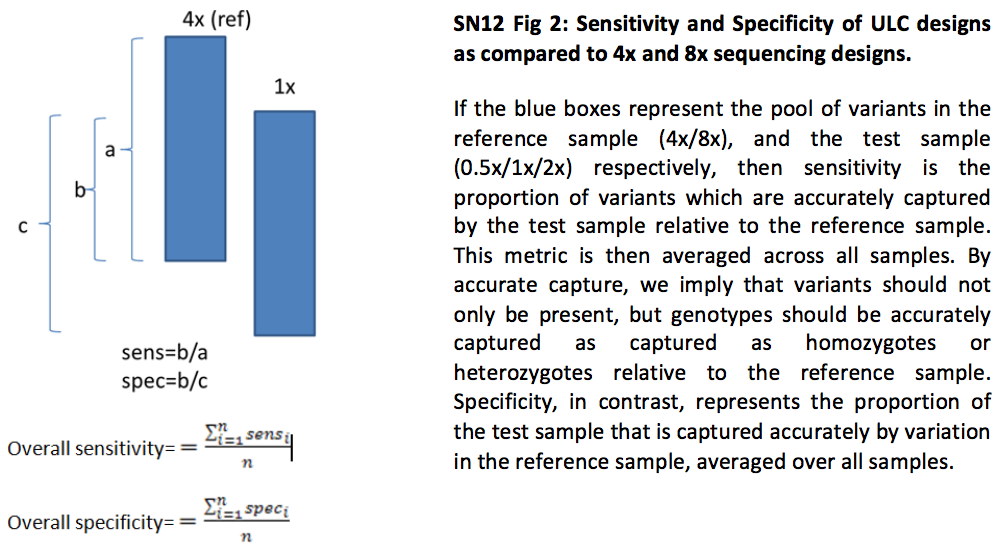
\includegraphics[trim={0 0 0cm 0},clip,width=0.9\textwidth]{fig/SN12f2}
\caption[Sensitivity and specificity as compared between higher and lower coverage sequence data.]{The blue boxes represent the pool of variants in the reference sample (4x/8x), and the test sample (0.5x/1x/2x) respectively. Sensitivity is the proportion of variants which are accurately captured by the test sample relative to the reference sample. This metric is then averaged across all samples. By accurate capture, we imply that variants should not only be present, but genotypes should be accurately captured as homozygous or heterozygous relative to the reference sample. Specificity represents the proportion of the test sample that is captured accurately by variation in the reference sample, averaged over all samples.}
\label{fig:SN12f2}
\end{figure}